\documentclass[
  ngerman,
  twoside,
  captions=tableheading,
  BCOR=.5cm,
  fontsize=11,
  ]{scrreprt}
\usepackage[utf8]{inputenc}
\usepackage[german]{babel}
\usepackage[T1]{fontenc}
\usepackage{amsmath}
\usepackage{amsfonts}
\usepackage{amssymb}
\usepackage{lscape}
\usepackage{graphicx}
\usepackage{multirow}
\usepackage{lmodern}
\usepackage[left=2cm,right=2cm,top=2cm,bottom=2cm]{geometry}

\usepackage{biblatex}
\addbibresource{quellen.bib}

\begin{document}


\tableofcontents

\newpage

\chapter{Typischer Ablauf: Optische Litographie}
\begin{center}
\textbf{Vorbereitung}\\
$\downarrow$\\
Probe unter Mikroskop begutachten\\
$\downarrow$\\
\textbf{Probe reinigen}\\
$\downarrow$\\
\textit{Parallel dazu...}\\
\textbf{Maske einbauen/wechseln}\\
$\downarrow$\\
Probe unter Mikroskop begutachten\\
$\downarrow$\\
\textbf{Lack auftragen}\\
$\downarrow$\\
Probe unter Mikroskop begutachten\\
$\downarrow$\\
\textbf{Probe belichten}\\
$\downarrow$\\
\textbf{Photolack entwickeln}\\
$\downarrow$\\
Probe unter Mikroskop begutachten\\
$\downarrow$\\
\textbf{Fertig}
\end{center}

\begin{center}
\underline{\textbf{Probe unter Mikroskop begutachten:}}
\end{center}

Prinzipiell sollte nach jedem Schritt, der die Probe betrifft, die Oberfläche kontrolliert werden. Falls Dreck/Kratzer/Aceton- oder Iso-Rückstände oder ähnliches sichtbar sind, dann immer Bilder davon machen. Dies dient der späteren Nachverfolgung von Dreck oder Fehlstellen im Lack oder auf der Probe und ist deshalb enorm wichtig, um den Prozessablauf auf mögliche Fehler bzw. nicht-optimale Prozesse zu untersuchen. Außerdem kann so erkannt werden, wodurch mögliche Fehler im finalen Chip entstanden sein könnten und für die generelle Dokumentierung des Prozesses. 

\bigskip

\begin{center}
\underline{\textbf{1\,cm x 1\,cm Probenchips vs. Si-Wafer}}
\end{center}

Diese Anleitung ist primär auf die optische Litho mit 1\,cm x 1\,cm großen Proben ausgelegt. Wann immer sich ein Prozessschritt mit einem Si-Wafer relativ stark von dem des 1\,cm x 1\,cm-Chips unterscheidet, ist dies ausdrücklich erwähnt.


\chapter{Vorbereitung}
\begin{itemize}
\item \textbf{Handschuhe} und \textbf{Mundschutz} anziehen.
\item \textbf{Stickstoff} und \textbf{Druckluft} im Nebenraum (1.120, Service 1) aufdrehen
\item \textbf{Belichtungsmaschine} (MaskAligner) einschalten (Benötigt ca. \textbf{20\,min} bis die Lampe aufgeheizt ist)

\begin{description}
\item 1) \textbf{On} drücken $\rightarrow$ (Fertig bei \textbf{ready})
\item 2) \textbf{CP} drücken (constant power)
\item 3) \textbf{Start} drücken $\rightarrow$ \textit{Dauert nun ca. 20\,min}
\end{description}
(Benötigt später nach dem Ausschalten ebenfalls ca. 25\,min bis die Lampe abgekühlt ist)

\item \textbf{Vakuumpumpe} einschalten (Links unten vom MaskAligner; Gelber Knopf an der Pumpe)
\item \textbf{Reinraumtücher} auf Arbeitsfläche auslegen (2 große sollten für den Anfang reichen)
\item \textbf{Pinzette} (Siehe Abb.\ref{Pinzetten} welche) zuerst mit Aceton und dann mit Iso-Propanol mit einem Reinraumtuch säubern und auf Reinraumtücher ablegen.
\item \textbf{Heizplatte} einschalten. Anschließend die benötigte Zieltemperatur durch Drücken der \textbf{Set}-Taste (gedrückt halten) und den \textbf{Pfeiltasten} einstellen.\\

\textbf{Hinweis:} Die Zieltemperatur der Heizplatte von bspw. 90\,$^o$C ist bereits nach ca. 5-10\,min erreicht. Sollte man wissen, dass es deutlich länger braucht, bis man den Lack ausbacken kann, kann die Heizplatte auch erst später eingeschaltet werden.
\end{itemize}

\begin{figure}[h]
\centering
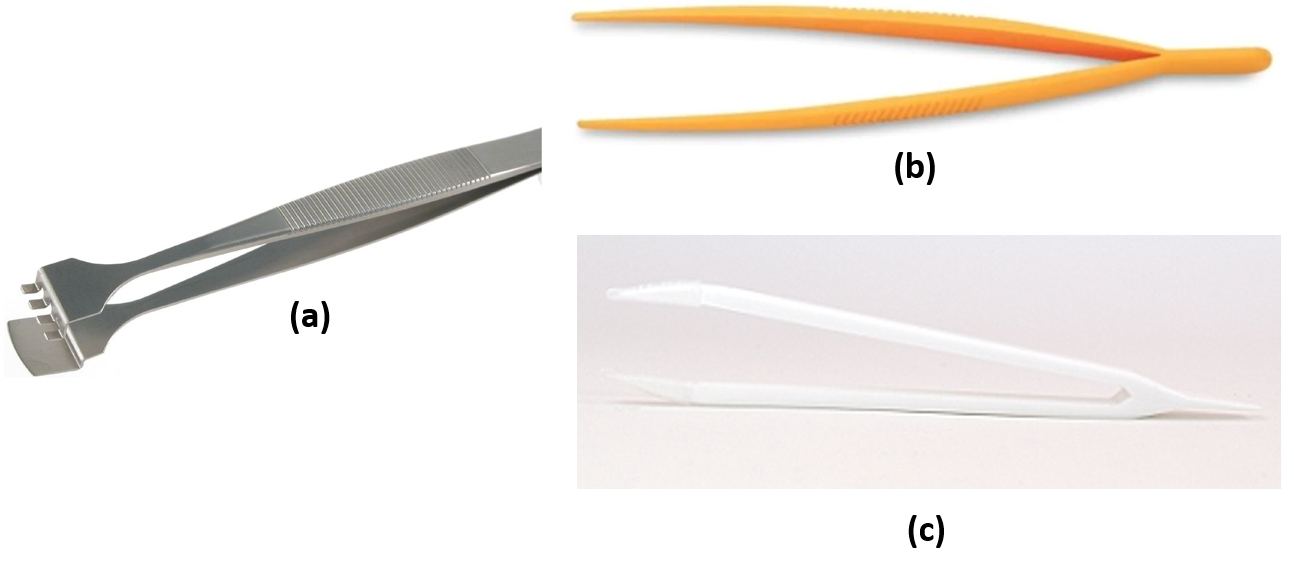
\includegraphics[scale=0.5]{Bilder/Pinzetten_combined.PNG}
\caption{Pinzetten im Litho-raum. \textbf{(a)} Wafer-Pinzette für Si-Wafer. \textbf{(b)} und \textbf{(c)} Pinzetten für 1\,cm x 1\,cm große Proben \cite{Kristallierschale, Petrischale}.}\label{Pinzetten}
\end{figure}

\newpage

\chapter{Probe reinigen}
\begin{center}
\begin{tabular}{| p{5cm} | p{10cm} |} \hline
\textbf{5 Kleine Gläschen}  & 2 für Aceton und 3 für Iso-Propanol\\
(s. Abb.~\ref{Reinigungsgläser}) & (Gläschen beschriften bzw. irgendwie unterscheiden!)\\ \hline
\textbf{1 Großes Glas} & Für das Aceton und Iso-Propanol Rest-Gemisch (Engl.: Waste)\\ \hline
\multicolumn{2}{|p{15cm}|}{\textbf{Pinzette, 2 große Reinraumtücher, Schutzbrille(!), Aceton- und Isopropanol-Spritzflaschen}} \\ \hline
\end{tabular}
\end{center}

\begin{tabular}{l p{14cm}}
\underline{Bemerkung:} & Vor und nach dem Reinigen \textbf{Bilder vom Chip von wichtigen Stellen} am Mikroskop abspeichern, um später nachverfolgen zu können, woher Dreck/kaputte Stellen kommen (könnten).
\end{tabular}

\begin{figure}[h]
\centering
\includegraphics[scale=0.6]{Bilder/Reinigungsgläser.PNG}
\caption{Gläser für die Reinigungsstraße. \textbf{(a)} Kristallisierschale für 1\,cm x 1\,cm große Chips bzw. \textbf{(b)} Petrischale aus Glas für Si-Wafer.}\label{Reinigungsgläser}
\end{figure}

\begin{description}
\item 1) \underline{Gläschen Reinigen:}\\
2 große \textbf{Reinraumtücher} auf der Arbeitsfläche auslegen und die \textbf{5 benötigten Gläschen} ordentlich mit \textbf{Reinstwasser} ausspülen. Dann zwei Gläschen mit \textbf{Aceton} bzw. 3 mit \textbf{Isopropanol} ausspülen und zum Trocknen gemäß der \textbf{Reinigungsstraße} in Abb.~\ref{Reinigungsstraße} ablegen.

\begin{figure}[h]
\centering
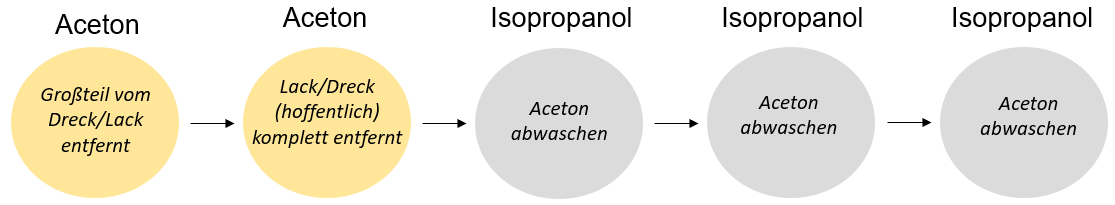
\includegraphics[scale=0.6]{Bilder/Ace_Iso_Schema.PNG}
\caption{Reinigungsstraße bestehend aus 2 Gläschen für Aceton und 3 für Iso-Propanol.}\label{Reinigungsstraße}
\end{figure}

\item 2) \underline{Mit Aceton reinigen:}\\
Probe mit \textbf{Pinzette} nehmen, die Oberfläche der Probe \textbf{dauerhaft mit Aceton benetzen} und währenddessen in das erste Aceton-Gläschen legen. Etwas mit Aceton auffüllen, sodass die Probe ordentlich bedeckt ist.\\
(Optional: Probe für bspw. 5\,Minuten ins Ultraschallbad stellen)\\

\underline{\textbf{Wichtig:}} Niemals das Aceton am Chip trocknen lassen ($\rightarrow$ Sonst \textbf{Schlierenbildung})
\begin{center}
\textit{Schritt noch einmal mit zweitem Gläschen wiederholen}
\end{center}

\item 3) \underline{Aceton mit Isopropanol abwaschen:}\\
Probe im zweiten Aceton-Gläschen mit der Pinzette festhalten und während dem Herausnehmen \textbf{permanent mit Isopropanol} benetzen. Die Probe wenige Sekunden mit Isopropanol abspritzen und währenddessen ins erste Isopropanol-Gläschen legen. Dieses anschließend ein wenig mit Isopropanol auffüllen, bis die Probe bedeckt ist.\\
(Optional: Probe für bspw. 5\,Minuten ins Ultraschallbad stellen)\\

\underline{\textbf{Wichtig:}} Auch hier das Isopropanol nicht auf der Probe trocken werden lassen, da sich sonst ebenfalls Schlieren bilden können!
\begin{center}
\textit{Diesen Schritt mit den übrigen 2 Gläschen wiederholen}
\end{center}

\item 4) \underline{Probe trocknen}\\
Probe aus dem letzten Isopropanol-Gläschen nehmen, dabei mit Isopropanol \textbf{abspülen}, auf einen sauberen Bereich eines \textbf{Reinraumtuchs ablegen} und ordentlich mit \textbf{Strickstoff trocken} pusten. Hierbei optimalerweise die Probe nicht mit der Pinzette festhalten sondern senkrecht von oben pusten, sodass die Probe nicht wegfliegt (Wäre schlecht).\\

\item 5) \underline{Kontrollieren}\\
Abschließend die Probe unter dem \textbf{Mikroskop begutachten}. Falls Unreinheiten oder Lackrückstände erkennbar sind $\rightarrow$ \textbf{Bilder machen}.
Diese mit Isopropnaol und/oder Wasser (Falls sich das anbietet; Bei YBCO bspw. nicht!) versuchen zu entfernen.\\
\textbf{Ansonsten: Reinigung wiederholen}\\
(Zuvor benutzte Aceton- und Isopropanol-Gläschen in Waste-Behälter entleeren und mit Aceton bzw. Isopropnaol entsprechend ausspülen!)

\end{description}

\newpage

\chapter{Maske einbauen}

\begin{description}
\item 1) Den benötigten \textbf{Maskenhalter} aus dem Schrank herausnehmen, am MaskAligner ablegen und den \textbf{Vakuumschlauch} anschließen.

\item 2) Die neu einzubauende \textbf{Maske} nehmen und unter dem Mikroskop begutachten. Falls rötliche Lackrückstände oder sonstiger Dreck auffällt, diesen versuchen mit Aceton, Iso-Propnaol und/oder Wasser (Falls dies möglich ist; bei YBCO nicht mit Wasser!) reinigen. Dabei zunächst ordentlich Aceton verwenden und die Maske möglichst permanent benetzt halten. Anschließend schnell das Aceton mit Iso-Propanol abwaschen und damit die Maske erneut ordentlich abspülen. Maske zur Seite auf ein Reinraumtuch oder zurück in die Verpackung ablegen. 

\item 3) Die beiden \textbf{seitlichen, großen Rädchen} am MaskAligner auf 10 stellen (Zentriert den Probentisch in der $x$-$y$-Ebene)

\item 4) \textbf{Vordere, kleine herausstehende Platte} durch vorderes, kleines Rädchen (auf der rechten Seite) mittig positionieren (Ermöglicht Rotation um $z$-Achse).
\item 5) \textbf{MaskAligern starten:}\\ 
Grüner Kippschalter auf \textbf{On} kippen $\rightarrow$ \textbf{Load} drücken $\rightarrow$ \textit{Miksoskop fährt herunter}\\
\textbf{Hinweis1:} Der MaskAligner kann nicht vor der anfänglichen Wartezeit von etwa 20\,min gestartet werden.\\
\textbf{Hinweis2:} Sollte das Mikroskop nicht herunterfahren, kann es durch Drücken von \textbf{F1} $\rightarrow$ \textbf{Enter} runtergefahren werden.

\item 6) \textbf{CHANGE MASK} drücken $\rightarrow$ \textit{Mikroskop fährt hoch}

\item 3) \textbf{Maske} mit der dunklen Seite (Chrom-Seite) nach oben so \textbf{positionieren}, dass die gewünschte Struktur möglichst mittig ist, die Maske aber dennoch von genügend Löchern durch das Vakuum angesogen wird.

\item 4) \textbf{Enter} drücken $\rightarrow$ \textit{Aktiviert (Deaktiviert) das Vakuum}\\
\textbf{Wichtig:} Testen, ob Maske wirklich korrekt angesogen wird!

\item 5) \textbf{Maskenhalter} nehmen und in den MaskAligner vorsichtig einsetzen. Währendessen mit einer Hand die angesogene Maske vor einem möglichen Fall schützen.\\
\textbf{Wichtig:} Jetzt \textbf{\underline{nicht Enter}} drücken, da sonst das Vakuum aufgehoben wird, die Maske dadurch nicht mehr angesogen wird und \textbf{runter fällt} $\rightarrow$ Kratzer in wichtigen Strukturen kann entstehen. 
\begin{center}
\textit{(Gilt nur solange man im CHANGE-MASK-Modus ist)}
\end{center}

\item 7) \textbf{CHANGE MASK} drücken $\rightarrow$ \textbf{Fertig}
\end{description}

\chapter{Maske ausbauen}
\begin{description}
\item 1) \textbf{CHANGE MASK} drücken $\rightarrow$ hebt die Fixierung des Maskenhalters im MaskAligner auf.

\item 2) Maskenhalter vorsichtig aus dem MaskAligner heraus nehmen und seitlich auf die dafür vorgesehene Ablagestele ablegen.

\item 3) \textbf{Enter} drücken $\rightarrow$ Vakuum wird aufgehoben. 

\item 4) Maske vom Maskenhalter nehmen und in die entsprechende Verpackung legen.

Neue Maske einbauen? $\rightarrow$ Siehe 4.\\
MaskAligner ausschalten? $\rightarrow$ Siehe 8.\\

\end{description}


\newpage

\chapter{Lack auftragen}

\begin{tabular}{| p{5cm} | p{10cm} |} \hline
\textbf{Pipette und Pipettenaufsätzen} & Befinden sich im Glas-Regal rechts hinten im Raum\\ \hline
\textbf{Benötigter Lack} & Befindet sich auf im Glas-Regal.\newline
\textbf{Achtung:} Lack vorsichtig und langsam rübertragen!\\ \hline
\textbf{Großes Glas} & Zum Zwischenlagern der Pipette\\ \hline
\textbf{Metallplatte} & Zum Abkühlen des Chips und damit sich der Lack anpassen kann\\ \hline
\textbf{Spincoater} und \textbf{Heizplatte} & Heizplatte sollte bereits nach Betreten des Litho-Raums auf die gewünschte Temperatur gestellt werden.\\ \hline

\end{tabular}

\bigskip

\begin{description}
\item 1) \textbf{Spincoater zusammenbauen}

\item 2) \textbf{Schleuder einschalten} (grüner Kippschalter)\newline
$\rightarrow$ Warten, bis alle Tests durchlaufen sind und die Fehlermeldung \textbf{Empty Battery} erscheint\newline
$\rightarrow$ Zum Quittieren \textbf{Enter} drücken

\item 3) \textbf{Rezept} einprogrammieren:\newline
\textbf{Edit} $\rightarrow$ (Edit Menu) $\rightarrow$ \textbf{Edit} $\rightarrow$ (A blinkt) $\rightarrow$ mit \textbf{Shift} rechts auf \textbf{Edit} (Um das Rezept zu ändern) $\rightarrow$ \textbf{Enter} $\rightarrow$ \textbf{EDIT} $\rightarrow$ \textbf{Enter} $\rightarrow$ Gewünschte Parameter eingeben (Jeweils mit \textbf{Enter} bestätigten)\\
\begin{center}
\begin{tabular}{|l | c | l|}\hline
\textbf{Parameter} & \textbf{Beispiel} & \textbf{Beschreibung}\\ \hline
rpm & 6000 & rotations per minute\\
Ramp & 10 & Zeit, um auf gewünschte rpm zu kommen\\
Out & & Keine Angabe\\
Time & 40 & Gesamte Schleuderzeit\\
E & n & Keine Angabe\\ \hline
\end{tabular}
\end{center}

\textbf{Zurück-Symbol} drücken $\rightarrow$ (Main MENU) $\rightarrow$ \textbf{Run} $\rightarrow$ \textbf{Run} $\rightarrow$ \textit{Rezept A auswählen} $\rightarrow$ Mit \textbf{Enter} bestätigten

\item 4) \textbf{Lackschleuder Vakuum} drücken $\rightarrow$ \textit{Vakuum-Pumpe wird eingeschaltet}

\item 5) Rezept zunächst mit Dummy-Chip überprüfen
\begin{description}
\item i) Gummiring mittig platzieren und Dummy-Chip darauf legen 
\item ii) \textbf{Vakuum} drücken und überprüfen, dass Chip angesogen wird
\item iii) Mit \textbf{Start} oder \textbf{F1} Rezept starten und dabei Parameter überprüfen

\end{description}

\item 6) Aufsatz auf Pipette stecken, die Spitze mit Stickstoff reinigen, die zu entnehmende Menge durch Drehen an der Pipette einstellen und den Lack vorsichtig in die Pipette füllen. $\rightarrow$ Pipette auf größerem Glas zwischenlagern und Lackglas verschließen

\item 7) Etwas vom Lack aus Pipette entfernen, um Luftblasen zu vermmeiden, anschließend zügig den Lack auf die Probe auftragen und Rezept durch \textbf{Start} oder \textbf{F1} starten.

\item 8) Anschließend mit bloßem Auge und/oder am Mikroskop (Mit \textbf{Rotfilder}!) Lack auf glatte Oberfläche überprüfen\newline
\textbf{Hinweis:} Sollte der Lack Unregelmäßigkeiten (z.B. Schlieren) aufweisen, muss der Lack entfernt werden (Mit Aceton oder speziellen Lackentfernern), die Probe nochmal gereinigt werden und der Lack erneut aufgetragen werden.

\item 9) Sieht die Lackoberfläche gut aus, die Probe \textbf{einige Minuten} (Abhängig vom Lack $\rightarrow$ evtl. Liste vor Ort berücksichtigen) auf die Heizplatte legen und anschließend erneut \textbf{ca. 2-5min} auf der Kühlplatte auskühlen lassen.

\end{description}

\newpage

\chapter{Chip und Maske angleichen und belichten}
\begin{center}
\begin{tabular}{| l | c | l |}
\multicolumn{3}{c}{Unter \textbf{EDIT PARAMETER} veränderbare Einstellungen}\\ \hline
& Beispiel & \\ \hline
\textbf{Process:}  & Lithography & Prozess\\ \hline
\textbf{Exp. Time[s]:} & 4,5 & Belichtungszeit\\ \hline
\textbf{Al. Gap[$\mu m$]:} & 200 & Abstand \textit{Probe - Maske} 
während des Anpassens\\ \hline
\textbf{Expose Type:} & Hard & Probe wird an Maske gepresst\\ \hline
\textbf{HC Wait T.[s]:} & 2 & Keine Angabe\\ \hline
\textbf{WEC Type:} & Cont & Wedge Error Compensation\\ \hline
\textbf{N2 Purge:} & No & Yes : Stickstoff, No: Kein Stickstoff\\ \hline
\textbf{WEC Offset:} & Off & Keine Angabe\\ \hline
\end{tabular}
\end{center}

\begin{description}
\item 1) \textbf{Merken}, wo sich das benötigte Bild auf der Maske befindet.

\item 2) \textbf{Load} drücken $\rightarrow$ Schublade bis zum Anschlag herausziehen

\item 3) Probe nun \textbf{grob positionieren}, sodass Probe Löcher überdeckt und später angesogen werden kann

\item 4) \textbf{Enter} drücken $\rightarrow$ \textit{Probe wird angesogen (Dies auch überprüfen!)}

\item 5) Schubladen wieder einfahren und grob von oben schauen, ob Probe gut genug positioniert ist\newline

\underline{Sollte Probe und Bild zu weit entfernt liegen:}\\ 
\textbf{Probe neu positionieren:} \textbf{Unload} drücken $\rightarrow$ Schublade rausziehen $\rightarrow$ \textbf{Enter} drücken (Vakuum wird aufgehoben) $\rightarrow$ Position korrigieren $\rightarrow$ \textbf{Enter} drücken (Vakuum wird eingeschaltet) $\rightarrow$ \textbf{Load} drücken $\rightarrow$ Schublade einfahren\\
\textbf{Eventuell Maske neu positionieren:} Siehe 4.

\item 6) (Wenn Probe gut positioniert ist) $\rightarrow$ \textbf{Enter} drücken \newline 
$\rightarrow$ \textit{Probe wird an die Maske gepresst und dann den in \textbf{Al. Gap [$\mu m$]} gewählten Abstand von ihr entfernt.}

\textbf{Hinweis:} Sollte das Licht bei \textbf{BSA MICROSCOPE} leuchten,  sollte dieses nun ausgeschaltet werden.

\item 7) In das Mikroskop schauen und mit Pfeiltasten die Probe und das gewünschte Bild suchen (Geht schneller, wenn die Taste \textbf{FAST} gedrückt wurde). DIe Probe mit den seitlichen großen 2 Rädchen in x- und y-Richtung verschieben und mit dem kleineren Rädchen vorne rechts so um die z-Achse rotieren, bis Maske und Probe wie gewünscht übereinstimmen.\newline
\textbf{Hinweis:} Auf bereits bestehende Identifier achten, sollte einer vorhanden sein (Evtl. muss Probe neu positioniert werden $\rightarrow$ Siehe Schritt 5) )

\item 8) Mit \textbf{ALIGNN CONT/EXP} wird die Probe (Wie während des Belichtens auch) gegen die Maske gepresst. Nun kann überprüft werden, dass die Probe nicht beim Andrücken (Bspw. aufgrund unterschiedlich hoher Lackberge am Rand) verrutscht. ($\rightarrow$ Erneut \textbf{ALIGNN CONT/EXP} drücken, damit die Probe wieder entfernt wird.)

\item 9) Liegt Probe wie gewünscht $\rightarrow$ \textbf{Exposure} drücken $\rightarrow$ \textit{Startet die Belichtung}
\begin{center}
\textbf{Nicht in die austretende UV-Strahlung blicken!}
\end{center}

\item 10) \textbf{Unload} drücken $\rightarrow$ Schublade herausziehen $\rightarrow$ \textbf{Enter} drücken (Entfernt Sog) $\rightarrow$ Probe entfernen $\rightarrow$ Maske (Falls nicht mehr benötigt) wie in \textbf{5. Maske ausbauen} beschrieben entfernen.

\end{description}


\chapter{Entwickeln des Photolacks}

\begin{tabular}{| p{5cm} | p{10cm} |} \hline
\textbf{Entwickler} & Ist abhängig vom verwendeten Lack\newline
(Siehe Liste vor Ort im Logbuch, welche Entwickler beim verwendeten Lack genutzt wurden bzw. im Internet auf der Seite des Herstellers)\\ \hline
\textbf{2 Kleine Gläschen} & 1 Gläschen für den Entwickler und 1 Gläschen für hochreines Wasser\\ \hline
\textbf{Stoppuhr} & \\
\textbf{Schutzbrille!} & \\ \hline
\end{tabular}


\begin{description}


\item 1) (Eventuell Temperatur und Luftfeuchtigkeit im Raum notieren)

\item 2) Beide Gläser mit Reinstwasser reinigen und eines mit selbigem auffüllen

\item 3) Anderes Gläschen mit Entwickler auffüllen (komplett, damit genügend Entwickler vorhanden ist) und beide Gläser beschriften bzw. markieren.

\item 4) Probe im Entwickler (Eventuell hochkant) eine gewisse Zeit (Vergleiche Liste vor Ort) gut \textbf{schwenken}, sodass die Probe permanent mit dem Entwickler in Kontakt kommt (Entwickler wird währendessen teilweise verbraucht)

\item 5) Anschließend Probe im Wasserglass kurz ausspülen und anschließend mit Stickstoff trocken blasen (Und eventuell 5-10 s auf Heizplatte trocknen lassen)

\item 6) Unter dem Mikroskop überprüfen, ob Struktur korrekt übertragen wurde und ob sich Fehler/Dreck gebildet haben (Falls grobe Fehler: Lack mit Aceton entfernen, ca. 15s auf Heizplatte trocknen lassen und Lack erneut auftragen)

\end{description}

\chapter{MaskAligner ausschalten}
\begin{description}
\item 1) Wenn sich keine Maske bzw. Maskenhalter mehr im MaskAligner befindet, diesen durch Umschalten des grünen Kippschalters auf \textbf{Off} ausschalten.

\item 2) Vakuum-Pumpe ausschalten. (Sollte sie noch an sein)

\item 3) \textbf{Wichtig: 20\,min} warten und dann erst die Belichtungsmaschine durch Drücken des \textbf{Off}-Knopfes ausschalten.

\item 4) \textbf{Stickstoff} und \textbf{Druckluft} im Service-Raum nebenan ausdrehen.
\end{description}



\begin{landscape}

\chapter{Übersichtstabelle}

\begin{tabular}{| l | l | l || l | l | l | l | l | l | l | l | l || p{7cm} |}\hline
\multirow{2}{*}{\textbf{Datum}} & 
\multirow{2}{*}{\textbf{Probe}} &  
\multirow{2}{*}{\textbf{Maske}} & 
\multirow{2}{*}{\textbf{Lack}} & 
\textbf{Ent-} & 
\multirow{2}{*}{$T_{Heiz}$} & 
\multicolumn{3}{| c |}{\textbf{Dauer [s]}} & 
\multicolumn{3}{| c |}{\textbf{Rezept}} & 
\multirow{2}{*}{\textbf{Kommentar}}\\ \cline{7-12}
& & & & \textbf{wickler} & & Heizpl. & Belicht. & Entw. & rpm & ramp & time & \\ \hline \hline
&&&&&&&&&&&&\\
&&&&&&&&&&&&\\ \hline
&&&&&&&&&&&&\\
&&&&&&&&&&&&\\ \hline
&&&&&&&&&&&&\\
&&&&&&&&&&&&\\ \hline
&&&&&&&&&&&&\\
&&&&&&&&&&&&\\ \hline
&&&&&&&&&&&&\\
&&&&&&&&&&&&\\ \hline
&&&&&&&&&&&&\\
&&&&&&&&&&&&\\ \hline
&&&&&&&&&&&&\\
&&&&&&&&&&&&\\ \hline
&&&&&&&&&&&&\\
&&&&&&&&&&&&\\ \hline
&&&&&&&&&&&&\\
&&&&&&&&&&&&\\ \hline
&&&&&&&&&&&&\\
&&&&&&&&&&&&\\ \hline
&&&&&&&&&&&&\\
&&&&&&&&&&&&\\ \hline
&&&&&&&&&&&&\\
&&&&&&&&&&&&\\ \hline
&&&&&&&&&&&&\\
&&&&&&&&&&&&\\ \hline
&&&&&&&&&&&&\\
&&&&&&&&&&&&\\ \hline
&&&&&&&&&&&&\\
&&&&&&&&&&&&\\ \hline
&&&&&&&&&&&&\\
&&&&&&&&&&&&\\ \hline


\end{tabular}

\end{landscape}

\printbibliography

\end{document}